\section{Architecture}
\begin{frame}
    \frame{\frametitle{Generative Adversarial Networks - Architecture}}
	% \myheading{Module 23.2: Generative Adversarial Networks - Architecture}
\end{frame}

\begin{frame}
	\begin{itemize}
		\item<1-> We will now look at one of the popular neural networks used for the generator and discriminator (Deep Convolutional GANs)
		For discriminator, any CNN based classifier with 1 class (real) at the output can be used (e.g. VGG, ResNet, etc.)
	\end{itemize}
	\visible<1->{
		\begin{center}
		\begin{figure}
          \hyperlink{DCGAN}{
			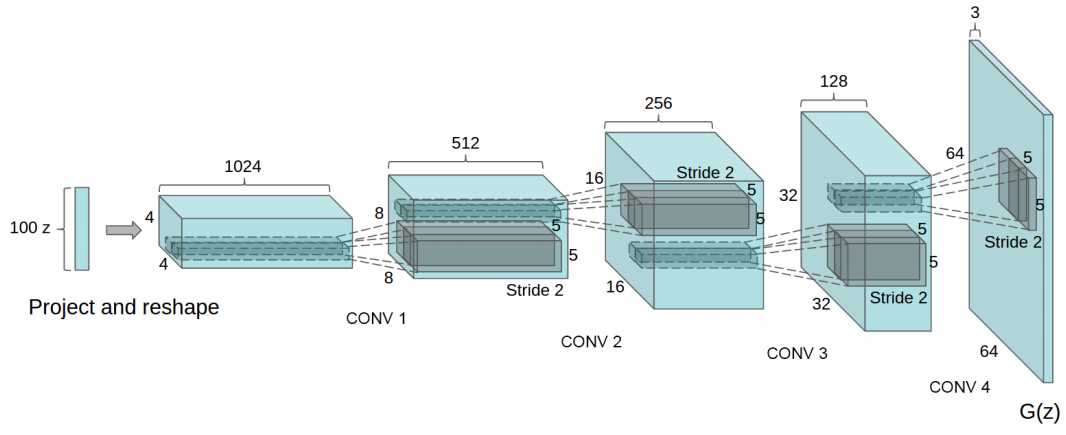
\includegraphics[scale=0.21]{images/dcgan_gen.png}
			\caption{Generator (Redford et al 2015) (left) and discriminator (Yeh et al 2016) (right) used in DCGAN}
          }
		\end{figure}
		\end{center}
	}
\end{frame}

\begin{frame}
	Architecture guidelines for stable Deep Convolutional GANs
	\begin{itemize}
		\item Replace any pooling layers with strided convolutions (discriminator) and fractional-strided convolutions (generator).
		\item Use batchnorm in both the generator and the discriminator.
		\item Remove fully connected hidden layers for deeper architectures.
		\item Use ReLU activation in generator for all layers except for the output, which uses tanh.
		\item Use LeakyReLU activation in the discriminator for all layers
	\end{itemize}
    \hyperlink{miteshk}{
        \begin{figure}
            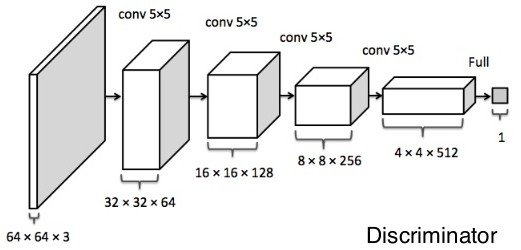
\includegraphics[scale=0.32]{images/dcgan_disc.jpg}
            \caption{Generator (Redford et al 2015) (left) and discriminator (Yeh et al 2016) (right) used in DCGAN}
        \end{figure}\
    }
\end{frame}

